\chapter{Result}
Now we can use our method to determine $dS/dt$, $Pre$, $ET$ and $R$. After that, we can combine these results and discuss the trend of water storage in Ob basin and the reason for it.
\section{Equivalent water height}
As mentioned in chapter 3, We have GRACE and GRACE-FO data from 4 data centers, which are CSR, GFZ, ITSG and JPL. We can plot the total water storage anomaly from 2002 to 2019. we can see in \ref{fig:4centers} that the trends of 4 curves suit each other well. By using the methods mentioned in \ref{sec:Gaussmarkov} we can generate one timeseries with their uncertainty in this period (\ref{fig:EWHs}).
\begin{figure}[htbp]
	\centering
	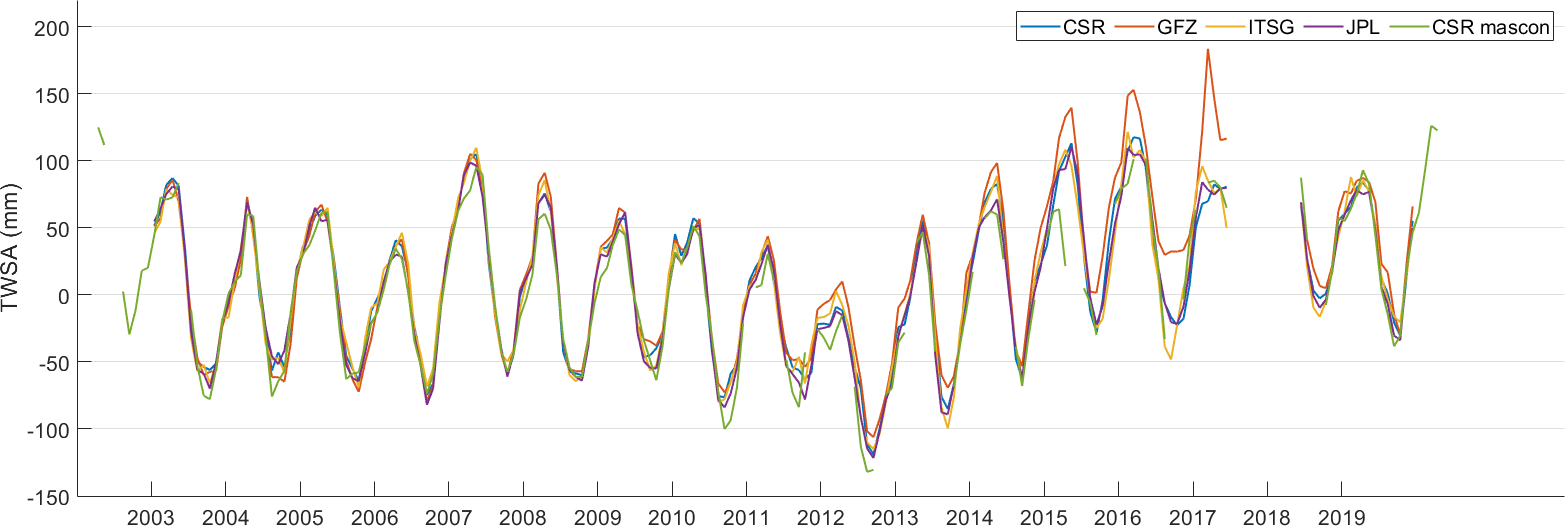
\includegraphics[width=0.9\textwidth]{TWSAall} % Datei in "bilder/" bei LaTeX: eps, bei PDFLaTeX: jpg (o.ä.) 
	\caption{Equivalent water height from CSR, GFZ, ITSG and JPL between 2002 and 2020} 
	\label{fig:4centers}
\end{figure}

% figure 4 data centers label(fig:4centers)

Since Ob basin is a quite big area, it is necessary to confirm if the behavior of the total water storage are identical in the whole area, we can divide the whole area in many grids \\

% text needs to be finished,  label(fig:grid of ob)

From the timeseries of the TWSA we see an obvious positive trend from 2013 to 2015. Thus, the whole period can divide into 3 phases. In order to find the changing points, we first plot the $dS/dt$ \ref{fig:dsdtall} by using the equation \ref{eq:dsdt}. With the help of the matlab functions \textit{movmean} and \textit{ischange} we can see the mean value of $dS/dt$ between 2013 and 2015 are much bigger than other periods, which confirms our assumption. This big change of the trend happened between October 2012 and September 2015.\ref{fig:dsdtmovmean} Therefore, we divide the whole timeseries into following 3 periods:\\\\
\begin{table}[htbp] \centering
	\begin{tabular}{|l|l|l|}
		\hline
		2003 - 2012 & 2013 - 2015 & 2015 - 2019 \\ \hline
	\end{tabular}
\end{table}\\
\begin{figure}[htbp]
	\centering
	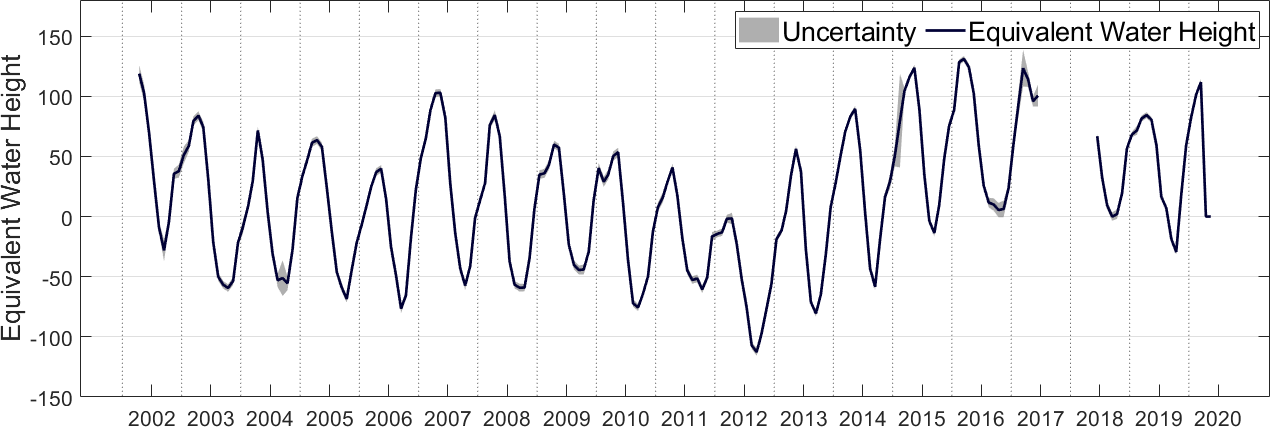
\includegraphics[width=0.9\textwidth]{EWH} % Datei in "bilder/" bei LaTeX: eps, bei PDFLaTeX: jpg (o.ä.) 
	\caption{Equivalent water height between 2002 and 2020} 
	\label{fig:EWHs}
\end{figure}
\begin{figure}[htbp]
	\centering
	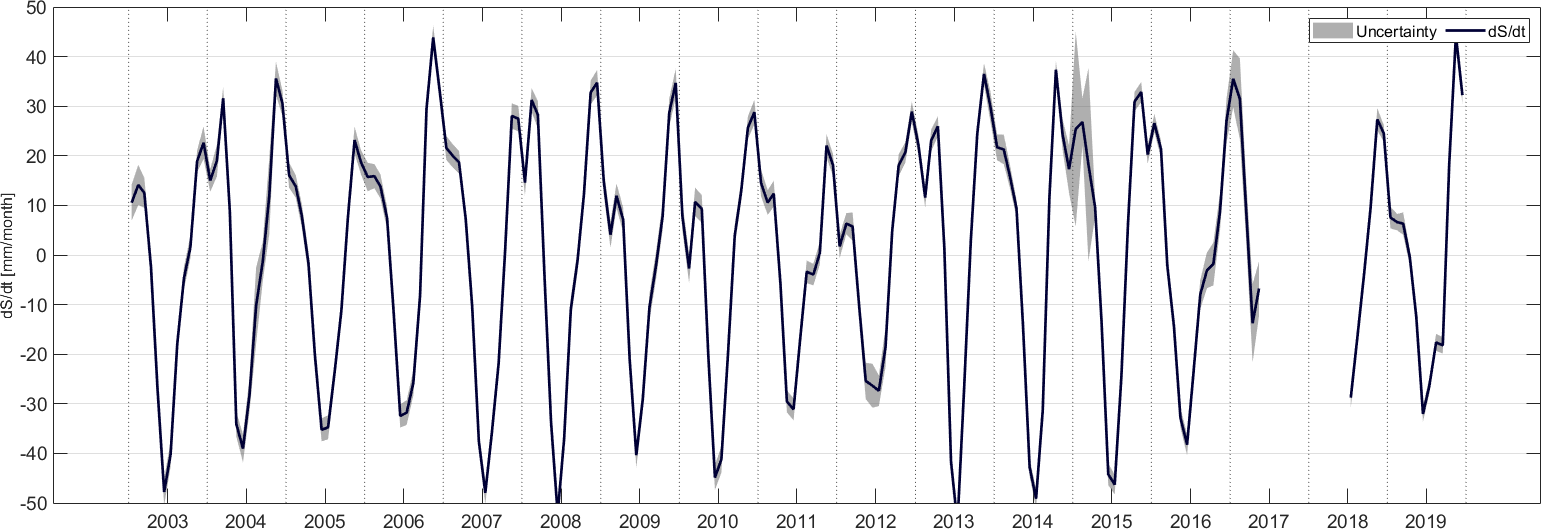
\includegraphics[width=0.9\textwidth]{dSdt} % Datei in "bilder/" bei LaTeX: eps, bei PDFLaTeX: jpg (o.ä.) 
	\caption{dS/dt between 2003 and 2020} 
	\label{fig:dsdtall}
\end{figure}
\begin{figure}[htbp]
	\centering
	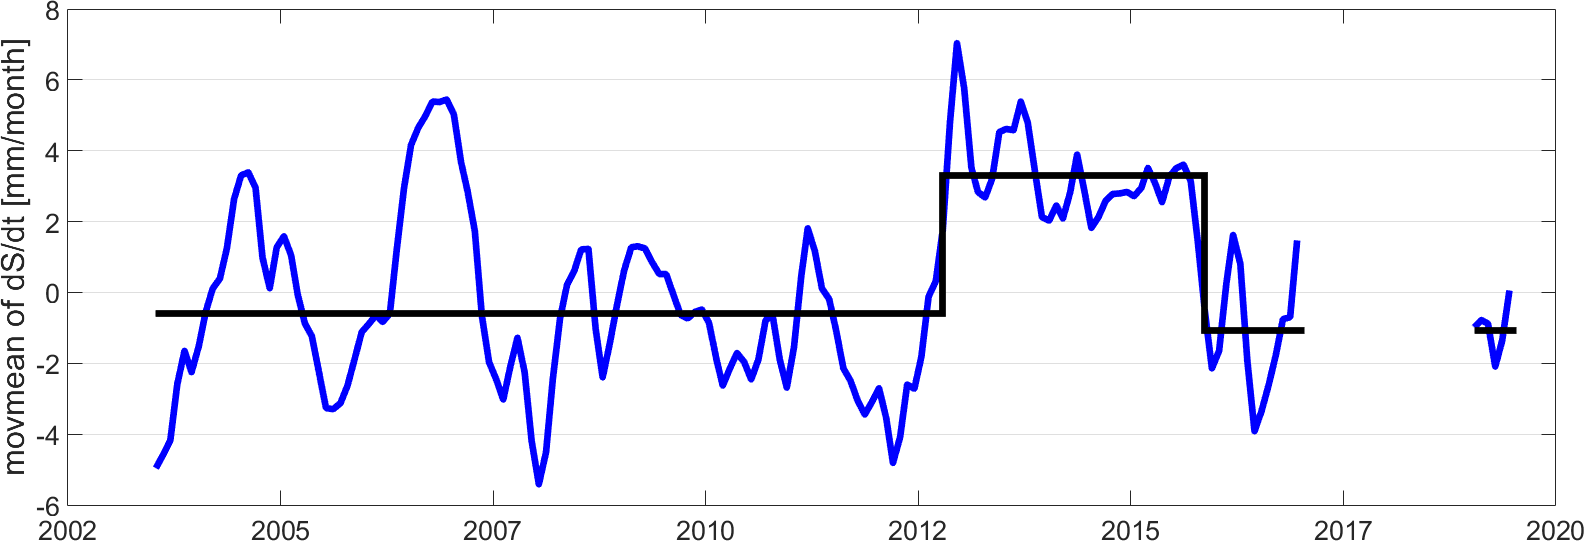
\includegraphics[width=0.9\textwidth]{dSdtmovmean} % Datei in "bilder/" bei LaTeX: eps, bei PDFLaTeX: jpg (o.ä.) 
	\caption{Sudden change of dS/dt between 2003 and 2020 after using movmean} 
	\label{fig:dsdtmovmean}
\end{figure}\\
% dsdt figure \label(fig:dsdtall)
Then, the mean value of $dS/dt$ with uncertainty in these 3 periods can be calculated. which can be seen as the trend of the total water storage change. However, it was a little tricky to do that for the periods because of the gap between GRACE and GRACE-FO. The data in 2017 and 2018 are partly lost. Therefore, instead by calculating the mean of dS/dt, we obtain the trend value by linear regression. The results are showed in \ref{fig:dsdtwithnum}
\begin{figure}[htbp]
	\centering
	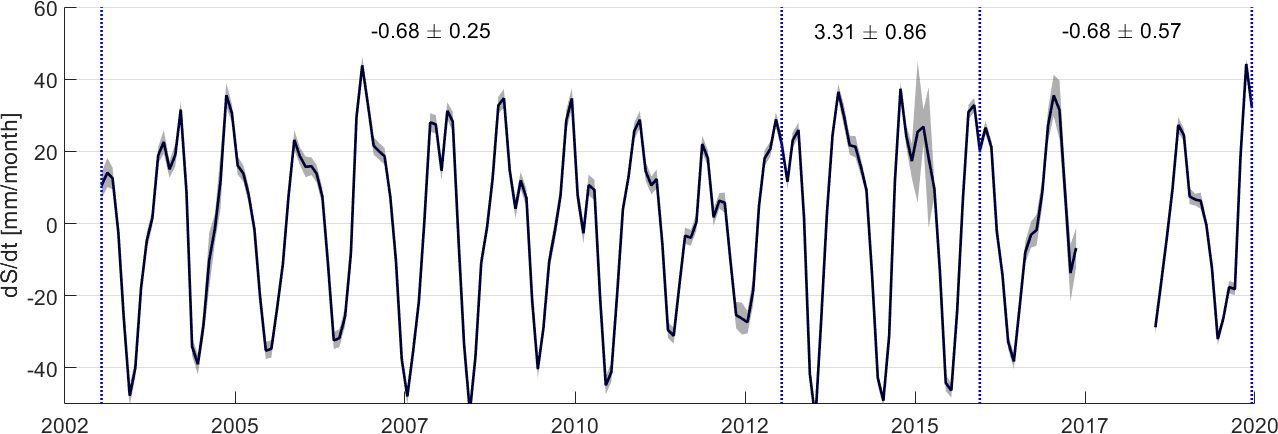
\includegraphics[width=0.9\textwidth]{dSdtwithnum} % Datei in "bilder/" bei LaTeX: eps, bei PDFLaTeX: jpg (o.ä.) 
	\caption{The mean value of dS/dt in three periods} 
	\label{fig:dsdtwithnum}
\end{figure}\\\\
From \ref{fig:dsdtwithnum} we can see, that the total water storage in the first and the third period are relative stable. However, between 2013 and 2015, the water in Ob river basin has gained from outside. 
\clearpage
\section{Precipitation}
It was mentioned in chapter 3 that we have precipitation data from 9 resources \ref{fig:precenter}, and one timeseries with uncertainty can be generated by combining them. The spatial behavior of precipitation in this area is also interesting to us. 
\begin{figure}[htbp]
	\centering
	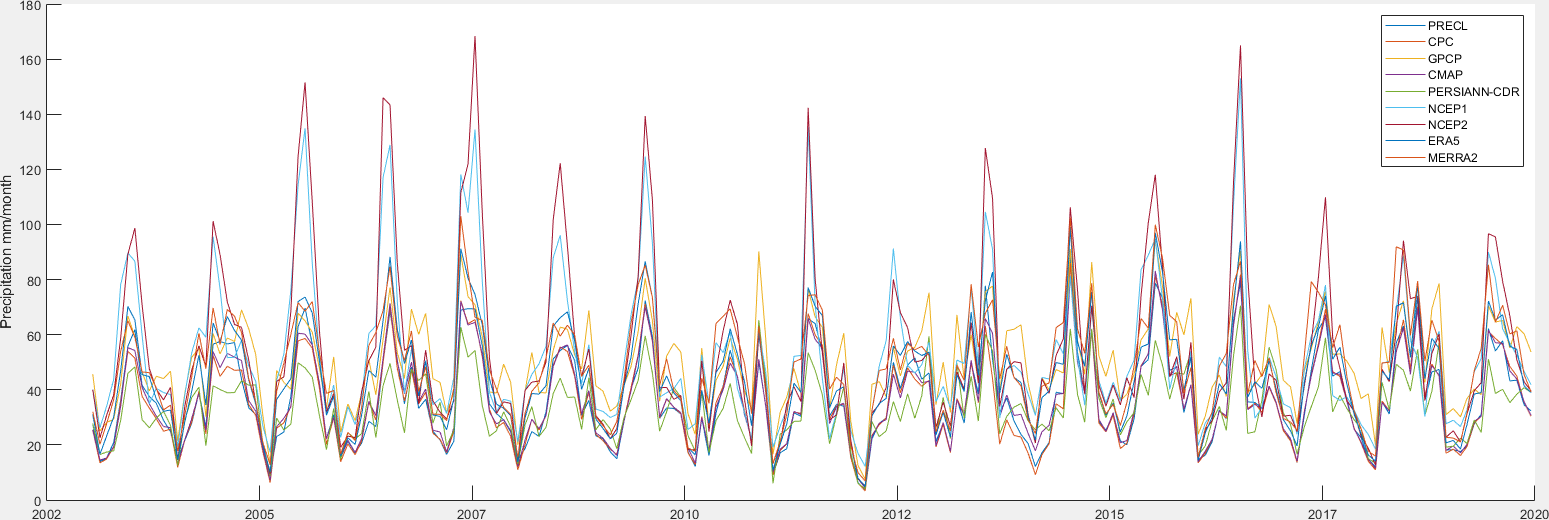
\includegraphics[width=0.9\textwidth]{precenter} % Datei in "bilder/" bei LaTeX: eps, bei PDFLaTeX: jpg (o.ä.) 
	\caption{Precipitation datasets} 
	\label{fig:precenter}
\end{figure}
\\
Since we have already divide the whole period into 3 phases, we are interested what we see the behavior of precipitations in this 3 phases. \ref{fig:allpre}
\begin{figure}[htbp]
	\centering
	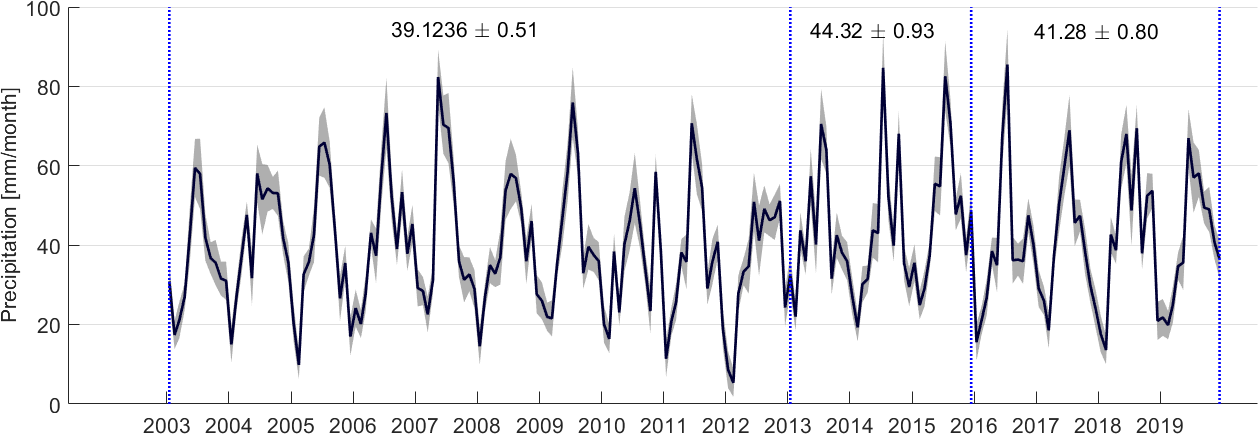
\includegraphics[width=0.9\textwidth]{precipitationwithnumber} % Datei in "bilder/" bei LaTeX: eps, bei PDFLaTeX: jpg (o.ä.) 
	\caption{precipitation with uncertainties between 2003 and 2020 and the mean value in 3 periods} 
	\label{fig:allpre}
\end{figure}
\\
We can see the precipitation in the second period is obviously higher than the other 2 periods.After 2016, the amount of precipitation has decreased. 
\clearpage
% all precipitation in one 
\section{Evatranspiration}
Just as precipitation, we present the evatranspiration temparally and spatially and cut the timeseries into 3 periods. 
\begin{figure}[htbp]
	\centering
	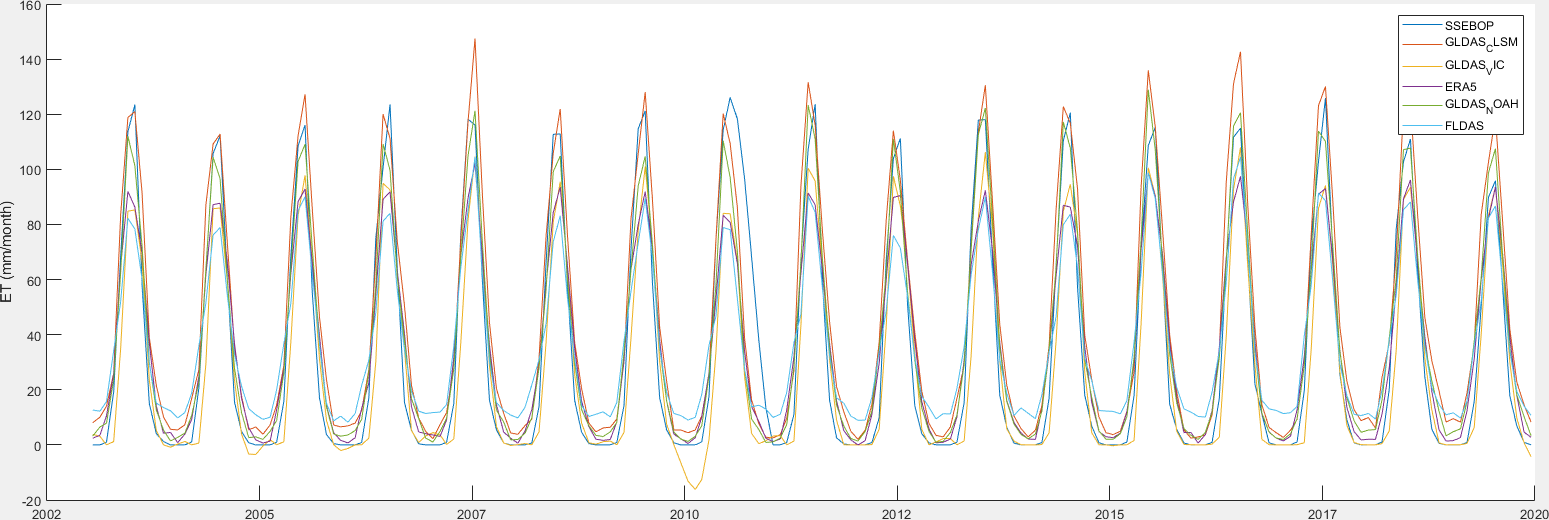
\includegraphics[width=0.9\textwidth]{etcenter} % Datei in "bilder/" bei LaTeX: eps, bei PDFLaTeX: jpg (o.ä.) 
	\caption{Evatranspiration datasets} 
	\label{fig:etcenter}
\end{figure}
\begin{figure}[htbp]
	\centering
	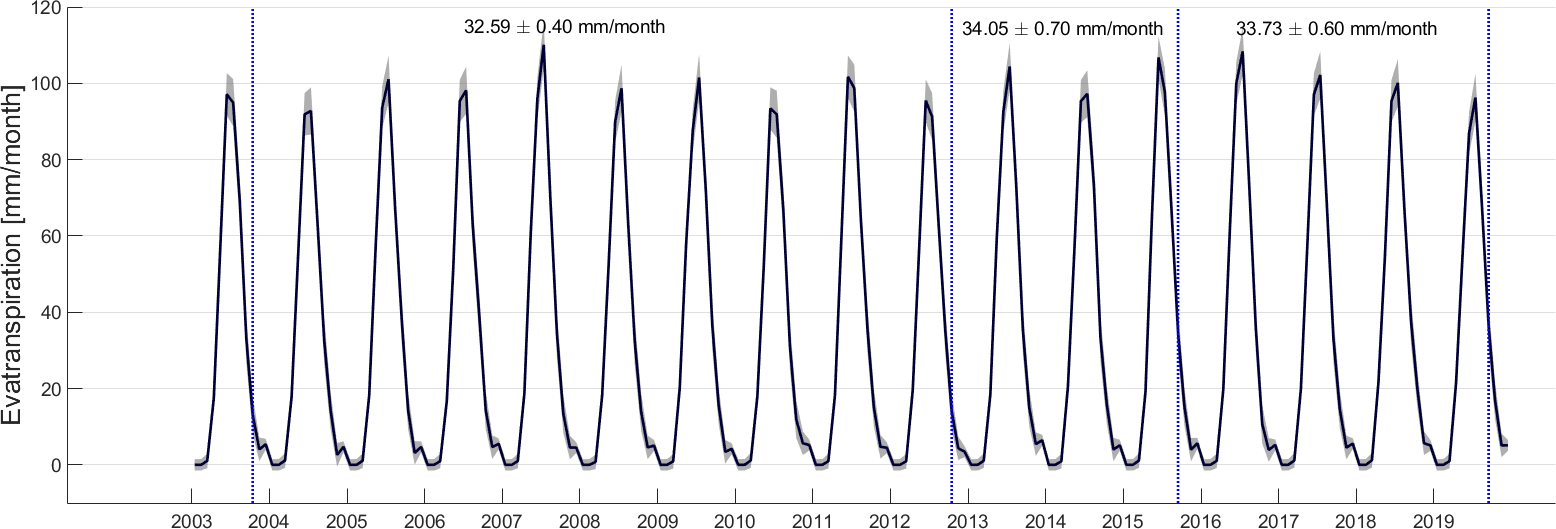
\includegraphics[width=0.9\textwidth]{etall} % Datei in "bilder/" bei LaTeX: eps, bei PDFLaTeX: jpg (o.ä.) 
	\caption{evatranspiration with uncertainties between 2003 and 2020 and the mean value in 3 periods} 
	\label{fig:etall}
\end{figure}
\\
The behavior of evatranspiration is similar to precipitation, in second period the evatranspiration reached the summit and then decreased, which suits theory of water cycle.  
\clearpage
\section{Runoff}
\subsection{Runoff from global datasets}
Like precipitation and evatranspiration, we have runoff data estimated from several models and meanwhile we have in-situ data till end of 2010. We can plot them in a way we did for precipitation and evatranspiration. From the \ref{fig:rcenter} we can assume that there are large differences between these models and in-situ. By calculating RMSE for these models \ref{tab:rmse} this assumption can be confirmed. The smallest RMSE for those daatsets are bigger than $8.18 \frac{mm}{month}$, which is far from what we needed.
\begin{figure}[htbp]
	\centering
	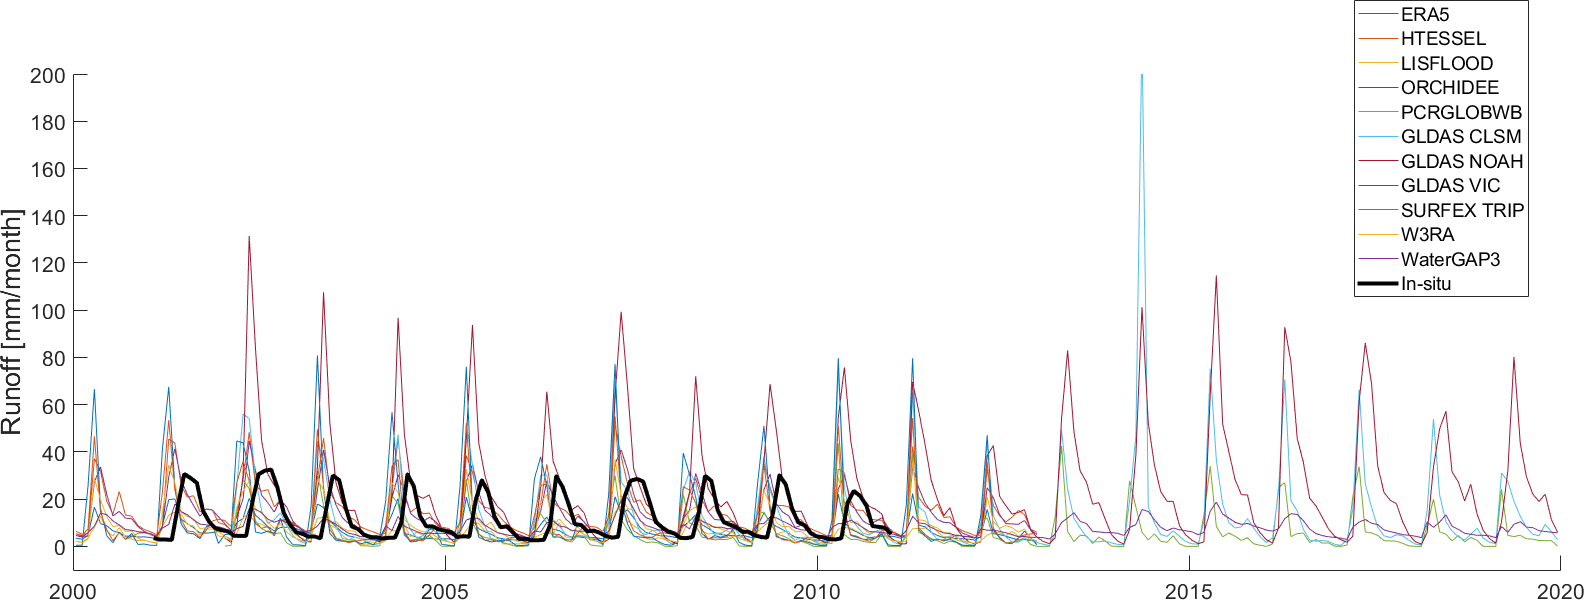
\includegraphics[width=0.9\textwidth]{runoffcenter} % Datei in "bilder/" bei LaTeX: eps, bei PDFLaTeX: jpg (o.ä.) 
	\caption{Runoff datasets} 
	\label{fig:rcenter}
\end{figure}
\begin{table}[htbp]\label{tab:rmse} \centering
	\begin{tabular}{|l|l|}
		\hline
		Datacenter  & RMSE (mm/month) \\ \hline
		ERA5        & 8.18  \\ \hline
		HTESSEL     & 10.40 \\ \hline
		LISFLOOD    & 11.92 \\ \hline
		ORCHIDEE    & 10.24 \\ \hline
		PCRGLOBWB   & 9.48  \\ \hline
		GLDAS CLSM  & 13.68 \\ \hline
		GLDAS NOAH  & 17.01 \\ \hline
		GLDAS VIC   & 25.95 \\ \hline
		SURFEX-TRIP & 22.05 \\ \hline
		W3RA        & 16.47 \\ \hline
		WaterGAP3   & 11.03 \\ \hline
	\end{tabular}
	\caption{RMSE for runoff datacenters}
\end{table}\\
Then, if we take the CDF of the difference from those models and in-situ data and set 10\% of mean in-situ runoff as quantile \ref{fig:rcdf} , it is shown that none of these datasets has achieved probability of 90\%
\begin{figure}[htbp]
	\centering
	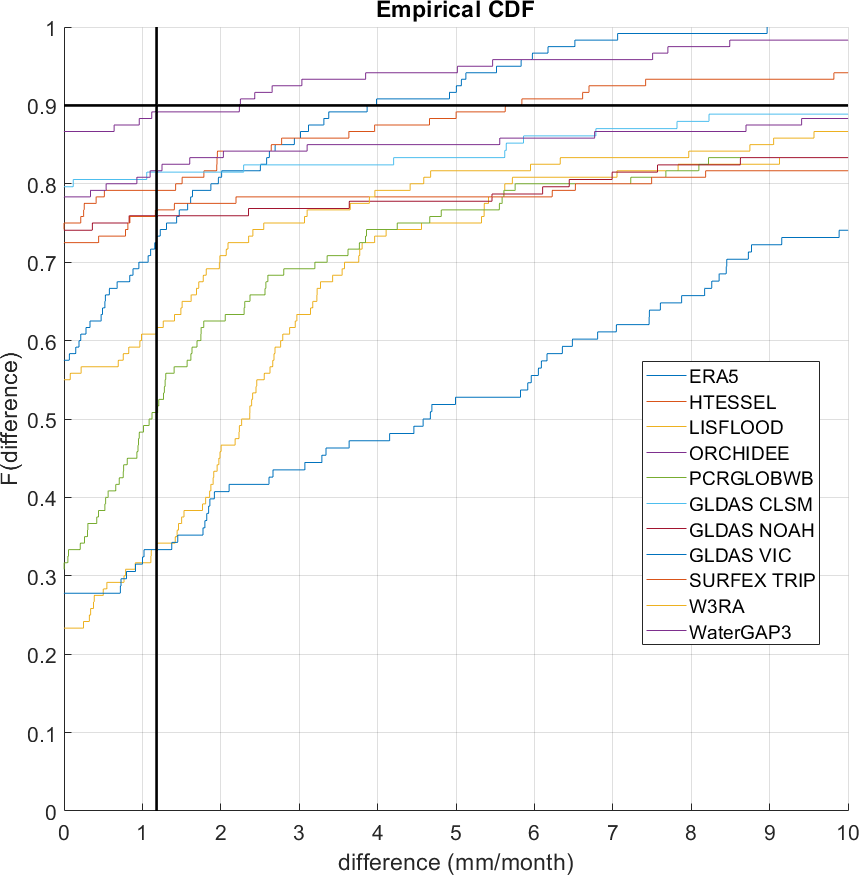
\includegraphics[width=0.6\textwidth]{rcdf} % Datei in "bilder/" bei LaTeX: eps, bei PDFLaTeX: jpg (o.ä.) 
	\caption{CDF of differences} 
	\label{fig:rcdf}
\end{figure}\\
\subsection{Estimating runoff using quantile function and satellite altimetry}
 As mentioned in \ref{sec:runoff}, we can use the satellite to determine the water level height in Ob river basin, and we also have the in-situ data, using the methods in \ref{sec:waterlevel}, the runoff can be estimated. We have chosen several virtual station for each satellite mission. After denying the virtual stations in bad locations we get 2 water level timeseries from Envisat, 2 from Saral and 2 from Sentinel. In order to get the most accurate runoff, we choose the water level timeseries from the virtual stations, which are closer to Salekhard, where the in-situ runoff are measured. \\\\
 In \ref{fig:waterlevel} the location of those virtual stations and the water level timeseries are represented. we finally choose the blue line from Envisat, the blue line from Saral and timeseries from Sentinel-3A to generate discharge.
 \begin{figure}[htbp]
 	\centering
 	\begin{minipage}[t]{0.7\textwidth}
 		\centering
 		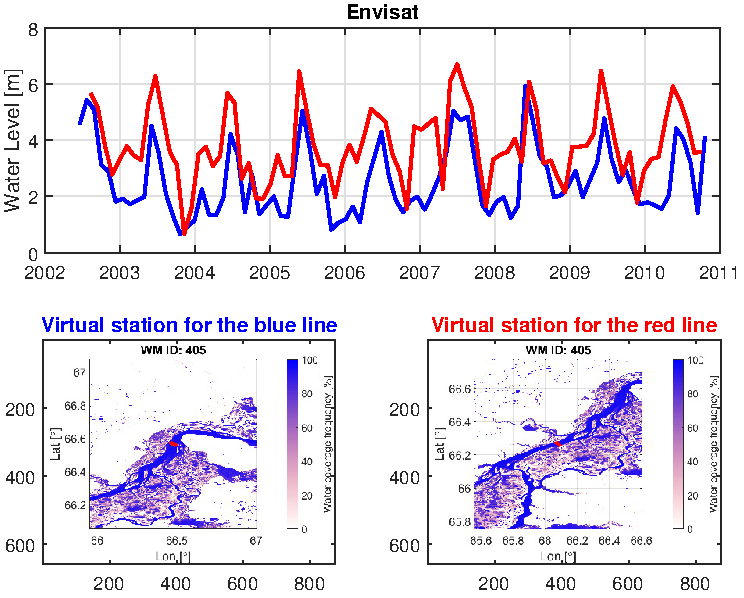
\includegraphics[width=0.8\textwidth]{Envisat_Ob} % Datei in "bilder/" bei LaTeX: eps, bei PDFLaTeX: jpg (o.ä.) 
 	\end{minipage}
 	\begin{minipage}[t]{0.7\textwidth}
 		\centering
 		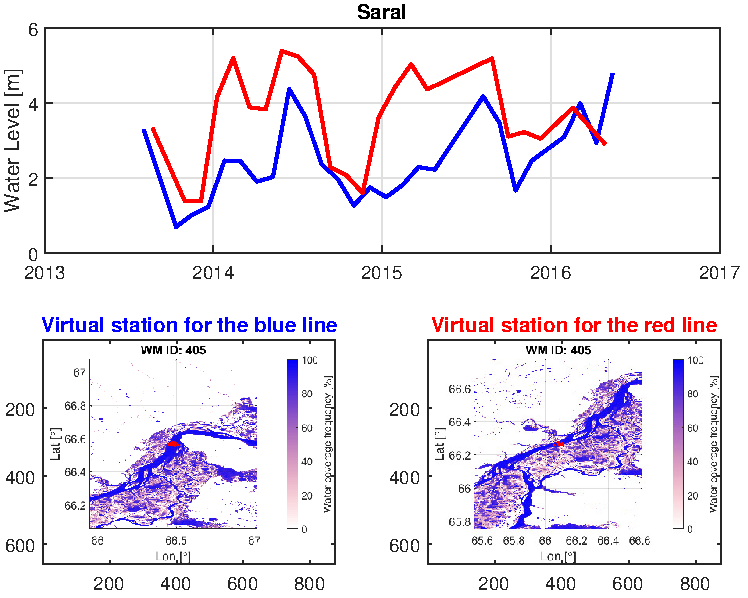
\includegraphics[width=0.8\textwidth]{Saral_Ob} % Datei in "bilder/" bei LaTeX: eps, bei PDFLaTeX: jpg (o.ä.) 
 	\end{minipage}
 \begin{minipage}[t]{0.7\textwidth}
 	\centering
 	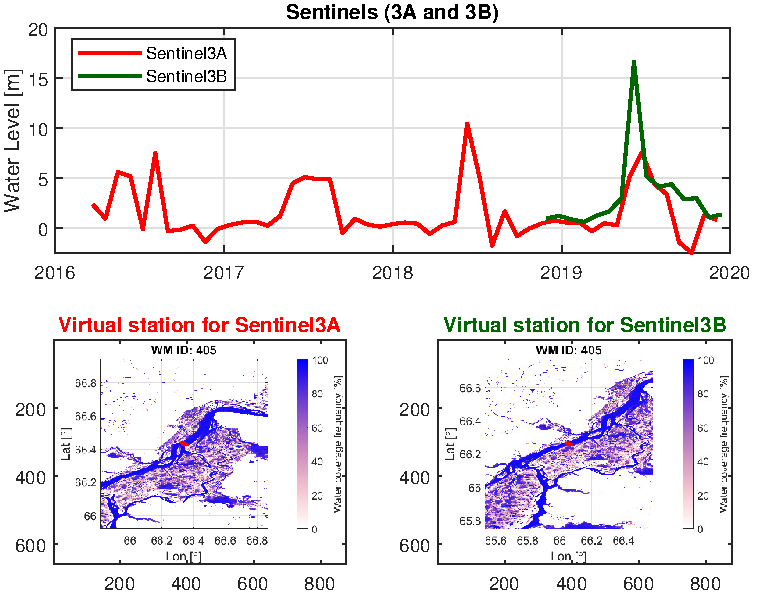
\includegraphics[width=0.8\textwidth]{Sentinels_Ob} % Datei in "bilder/" bei LaTeX: eps, bei PDFLaTeX: jpg (o.ä.) 
 \end{minipage}
 \caption{water level time series and the location of virtual station}
 \label{fig:waterlevel}
 \end{figure}
\\\\
Now we have in-situ runoff data from 2001 to 2010 and water level, Using the methods in \ref{sec:waterlevel}, we are able to find the probability connections between them and after all obtain a smoothened rating curve. We use this method for Envisat, Saral and Sentinel separetly and combine them in one time series. There are still several gaps in the series, we use interpolation to fill the gaps. Since we don't have uncertainty information for each month, we take the RMSE as the uncertainty for 3 periods.  
\begin{figure}[htbp]
	\centering
	\begin{minipage}[t]{0.9\textwidth}
		\centering
		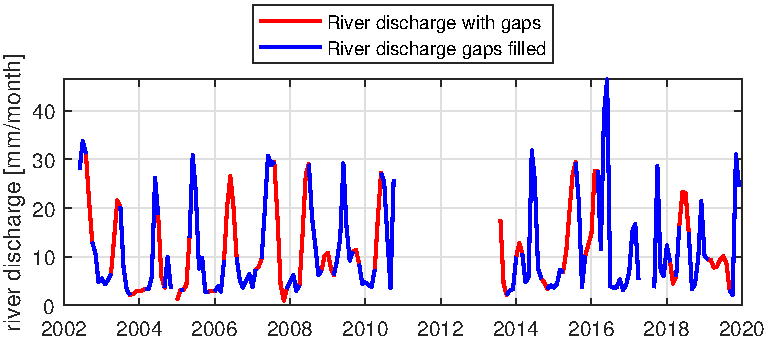
\includegraphics[width=1\textwidth]{Dis_Ob} % Datei in "bilder/" bei LaTeX: eps, bei PDFLaTeX: jpg (o.ä.) 
	\end{minipage}
	\begin{minipage}[t]{0.9\textwidth}
		\centering
		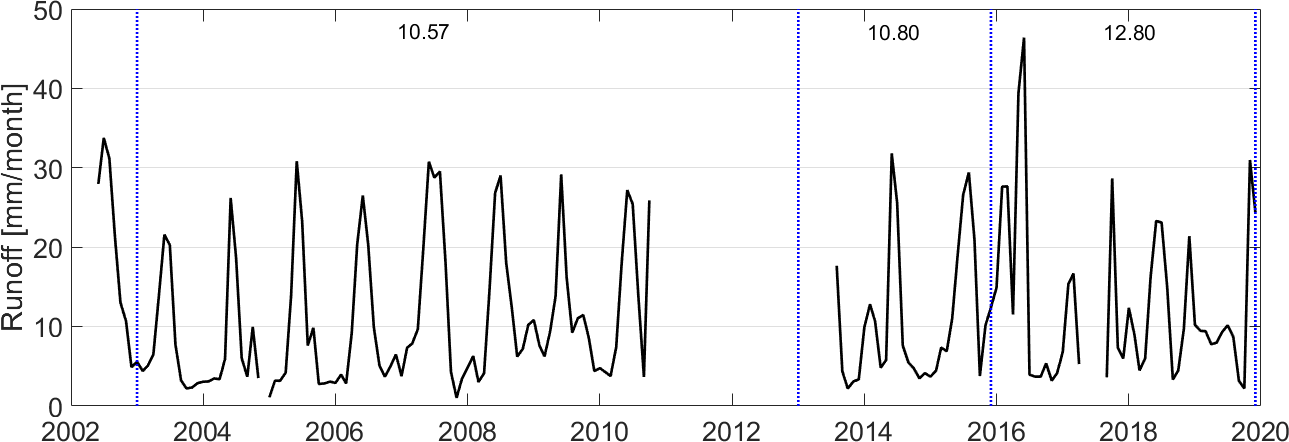
\includegraphics[width=1\textwidth]{runnumber} % Datei in "bilder/" bei LaTeX: eps, bei PDFLaTeX: jpg (o.ä.) 
	\end{minipage}
	\caption{runoff timeseries calculated from water level (up) and the mean value in 3 periods(bottom) }
	\label{fig:runoff}
\end{figure}
\clearpage
\section{Discussion about the quality}
Since the total water storage in the first period can be seen as stable, we take this period as the baseline for further analyze. Relative dS/dt, precipitaion, evatranspiration and runoff numbers of other 2 period are obtained based on that. \\\\
In any case, the equation of the water cycle has to be a true statement, which means the result of $Pre-\frac{dS}{dt}-ET-R$ should be 0. By setting results of both periods into this statement, it is shown that the results for the second period are proved while the results for the third periods are not ideal. This can be caused by the gap between GRACE and GRACE-FO. This gap is between Jul.2017 and May.2018, therefore, we only have full year data of 2016 and 2019 in this period. Though we tried linear regression to make the best use of what we have, this gap can still increase the instability of the final results because the period is not long enough. 
\begin{table}[htbp]\centering
	\begin{tabular}{|l|l|l|l|}
		\hline
		Period &  2003 - 2012 & 2013 - 2015 & 2016 - 2019  \\ \hline
		dS/dt            & $-0.68 \pm 0.25$     & $3.31 \pm 0.86$        & $-0.80 \pm 0.57$        \\ \hline
		Precipitaion               & $39.12 \pm 0.51$      & $44.32 \pm 0.93$       &$41.28 \pm 0.80$        \\ \hline
		Evatranspiration           & $32.59 \pm 0.38$       & $34.13 \pm 0.70$       & $33.78 \pm 0.6$        \\ \hline
		Runoff                     & $10.57  \pm 4.16$      & $10.80 \pm 4.16 $     & $12.80 \pm 4.16 $      \\ \hline
		\multicolumn{4}{|l|}{Based on the first period}                                         \\ \hline
		dS/dt           &             & $4.00 \pm 0.45$        & $-0.11 \pm 0.52$        \\ \hline
		Precipitaion               &             & $5.20 \pm 0.53$        & $2.15 \pm 0.61$         \\ \hline
		Evatranspiration           &             & $1.53 \pm 0.40$        & $1.19 \pm 0.46 $        \\ \hline
		Runoff                     &             & $0.23 \pm 2.94 $       & $2.23 \pm 2.94   $      \\ \hline
		Pre - dS/dt - ET - R &             & $-0.57 \pm 0.76$       & $-1.14 \pm 0.76 $    \\ \hline 
	\end{tabular}
	\caption{mean value of all water cycle component in 3 periods}
\end{table}